% !TeX root = ../libro.tex
% !TeX encoding = utf8

\chapter{Desarrollo e implementación}
En esta sección veremos cómo se han usado las técnicas y conceptos presentados para la realización de una aplicación web que permita al usuario crear e interactuar superficies a través de SDFs, ecuaciones implícitas y paramétricas. El motivo de desarrollar una aplicación web es que sea accesible al mayor número de usuarios y de la forma más cómoda posible. Se ha decidido usar \href{https://es.reactjs.org/}{React} para esta tarea, una biblioteca de JavaScript (y TypeScript) para interfaces de usuario. Es una librerçia muy popular, y por tanto muy bien documentada y con muchos paquetes de la comunidad disponibles. Las principales características de React son:
\begin{itemize}
    \item Utiliza la \textbf{extensión de sintaxis} JSX, la cual permite escribir código JavaScript como si se tratase de HTML o XML. Se pueden usar expresiones JSX dentro de bucles \texttt{for} o entornos condicionales \texttt{if}, y dentro de ellas se pueden agregar expresiones JS entre corchetes. 
    \item Se basa en \textbf{componentes autocontenidos y reutilizables}. La forma más común actualmente de declarar componentes es a través de funciones que reciben argumentos, o \texttt{props}, y devuelven una expresión JSX. Todos los componentes reciben el parámetro \texttt{children} por defecto, conteniendo la expresión JSX de los componentes que se encuentren entre las etiquetas de apertura y cierre del componente. El flujo de datos es unidireccional del componente padre a sus hijos.
    \item Utiliza un \textbf{DOM virtual} para solo actualizar los componentes cuyo estado o \texttt{props} han cambiado. En componentes funcionales, la manera de indicar variables que desencadenen un re-renderizado al ser modificadas es a través de \texttt{hooks}. En general, estos son funciones de JS que permiten crear y acceder al estado y ciclos de vida de React. Los principales son \texttt{useState}, usado para declarar una variable junto con su \textit{setter}, y \texttt{useEffect}, que permite ejecutar código cuando se actualice el componente. Si solo se quiere reaccionar a cambios de ciertos \textit{hooks} se puede indicar en las dependencias.
\end{itemize}

Un ejemplo de uso básico de JSX, componentes funcionales y manejo de estado sería el siguiente:
\begin{lstlisting}
function Tarjeta(props) {
  return (
    <div>
        {props.children}
        {props.nombre}
    </div>
  );
}

function Main() {
    const [miNombre, setMiNombre] = React.useState("Daniel");

    useEffect(()=>{
        console.log("Solo me ejecuto una vez al inicio");
    }, []);
    
    useEffect(()=>{
        console.log("Has cambiado el nombre");
    }, [miNombre]);
    
  return (
    <TarjetaNombre nombre={miNombre}>
      <h1>Hola, mi nombre es</h1>
    </TarjetaNombre>
  );
}
\end{lstlisting}

Las principales ventajas que aporta son:
\begin{itemize}
    \item La aplicación puede ser ejecutada en cualquier navegador, haciendo que sea mucho más accesible,
    \item Está basada en componentes modulares, lo que la hace escalable. Además. debido a su popularidad, hay una infinidad de librerías de terceros a nuestra disposición, ya sea específicas de React o de JavaScript.
\end{itemize}

% Un aspecto fundamental a lo largo de todo el desarrollo será el del rendimiento ya que las aplicaciones web solo tienen a su disposición una hebra de ejecución (la de interfaz de usuario), haciendo de cuello de botella para el resto de cálculos.\newline

La aplicación consta de tres componentes principales. Dos de ellos son con los que interactúa el usuario, uno en la que se le permite crear primitivas introduciendo directamente una SDF, ecuaciones implícitas o paramétricas, y otro que contiene un editor de nodos en forma de árbol para aplicar operaciones sobre las primitivas creadas y guardar los resultados obtenidos. El último componente actúa como gestor de almecenamiento y estado de la aplicación. A continuación estudiamos cada componente por separado describiendo los subcomponentes que la conforman y cómo estos interaccionan entre sí.


\section{Editor de nodos}
Este componente se base en \href{https://github.com/wbkd/react-flow}{React Flow}, un paquete muy completo que permite la implementación de diagramas interactivos basados en nodos. Cada nodo tendrá cierto número de puertos de entrada (solo permite la conexión con un nodo) y uno de salida (permite conectarse a varios nodos). Se nos permite declarar tipos de nodos según nuestras necesidades. Nosotros usaremos dos categorías principales de nodos.\newline

El \textbf{nodo de primitiva} es el más sencillo, y permite seleccionar una primitiva entre las guardadas para ser conectada a uno o varios nodos de operaciones.\newline

Los \textbf{nodos de operaciones} implementan las operaciones explicadas en la \autoref{sec:operaciones} y las aplican a las primitivas que reciben por sus puertos de entrada. A su vez hay cuatro tipos diferentes de estos nodos, uno por cada tipo de operación. Los nodos de operaciones de transformación, deformación y repetición tienen un único puerto de entrada, pues son operadores unarios. El nodo booleano sin embargo es capaz de recibir un número arbitrario de primitivas, ya que aunque los operadores booleanos son binarios, si se quiere realizar una misma operación de forma reiterada sobre varias primitivas puede ser muy tedioso. Así, si un nodo booleano recibe las primitivas $A_i$ con $i=1,\dots, n$, irá aplicando la operación de forma sucesiva sobre el resultado anterior según el orden de conexión. Por ejemplo, para la unión tendríamos
\begin{equation*}
    \bigcup_{i=0}^n A_i = A_n\bigcup (A_{n-1} \bigcup ( \cdots A_2 \bigcup A_1)).
\end{equation*}

La estructura de todos los nodos es similar. Todos cuentan con un encabezado que muestra de qué tipo son, un desplegable para elegir la primitiva u operación a usar seguido de un área con controles para los parámetros que pueda tener la primitiva y operación, un lienzo para mostrar el resultado de las operaciones aplicadas hasta el momento y un botón para contraer el nodo ocultando toda la información excepto el encabezado. Debido a esto tiene sentido tener un componente nodo general que se pueda adaptar a diferentes tipos de uso. El encabezado y elementos del desplegable se pasan fácilmente a través de \texttt{props}. Sin embargo para los parámetros sí que depende fuertemente del tipo de nodo en particular, y serán implementados por cada tipo de nodo por separado y pasado al general a través del parámetro \texttt{children}.\newline

Para gestionar el estado del editor de nodos usamos de nuevo Zustand, que principalmente contendrá la información de los nodos, las conexiones entre ellos, y varias funciones para gestionarlos (añadir, eliminar, actualizar, etc.). En particular, la información de cada nodo incluye su SDF, de forma que cuando un nodo detecta una nueva conexión en algún puerto de entrada se leen las SDFs de los nodos conectados y junto con los propios parámetros del nodo se actualiza la SDF del nodo. Cuando se elimina alguna conexión en el caso de los nodos diferentes al booleano simplemente la SDF pasa a ser indefinida, ya que solo tienen una entrada. En el caso del booleano habrá que tener en cuenta si todavía queda alguna entrada, reorganizar las restantes para que no haya puertos vacíos distintos al último, y reducir el número de puertos a uno menos. Para esto, se detecta la posición del puerto que se ha eliminado y se modifican las conexiones siguientes para cambiar su puerto al inmediatamente anterior. 
\begin{figure}[!h]
    \centering
    \begin{subfigure}[b]{0.45\textwidth}
        \centering
        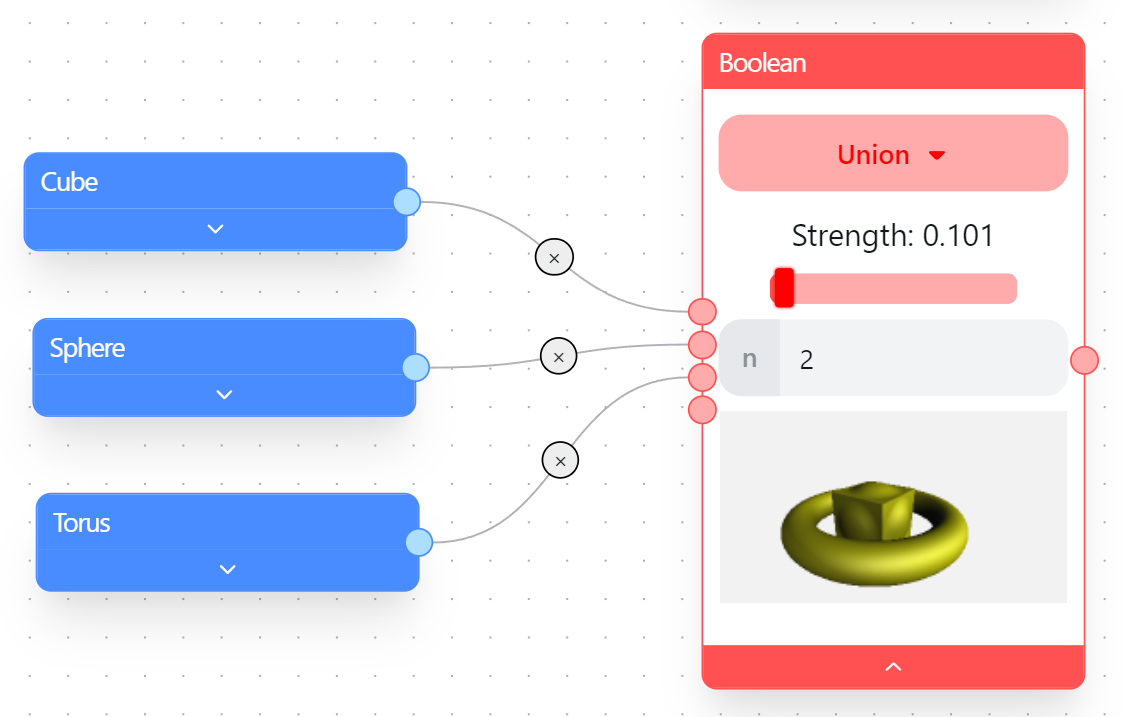
\includegraphics[width=\textwidth]{Plantilla-TFG-master/img/booleanBorrar1.png}
        \caption{Antes de eliminar}
    \end{subfigure}
    \hspace{15pt}
    \begin{subfigure}[b]{0.45\textwidth}
        \centering
        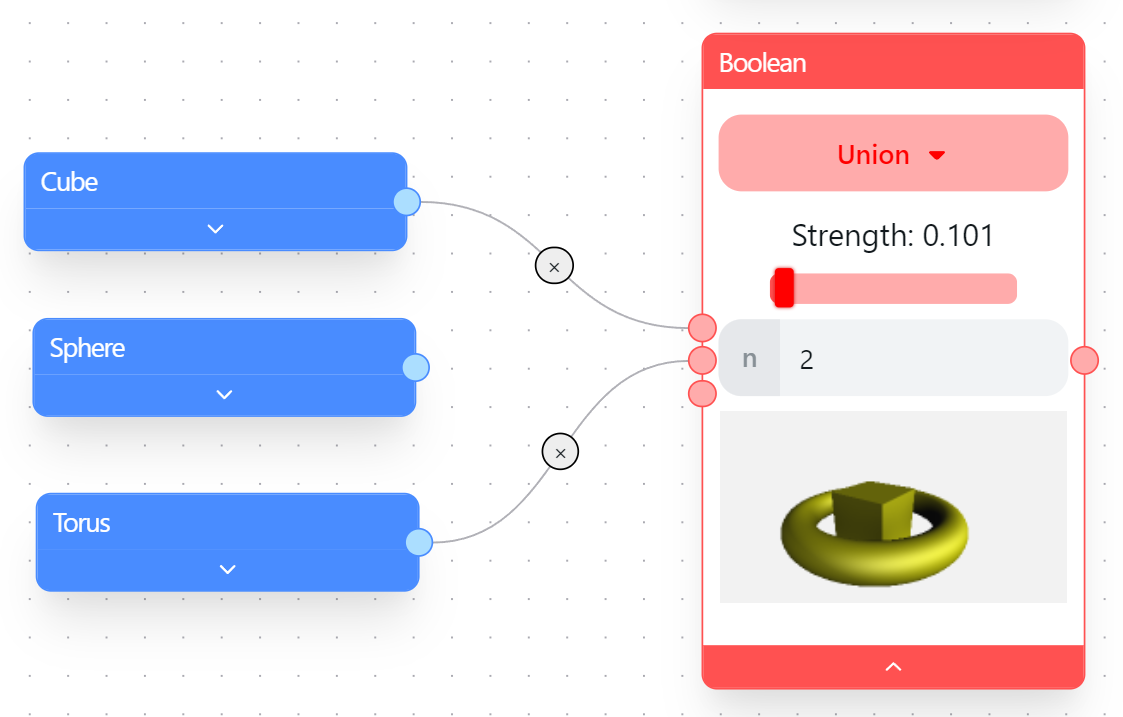
\includegraphics[width=\textwidth]{Plantilla-TFG-master/img/booleanBorrar2.png}
        \caption{Tras eliminar segunda conexión}
    \end{subfigure}
    \hfill
     \caption{Ejemplo de eliminación de conexión en nodo booleano}
\end{figure}

Cada nodo tiene una instancia de un componente \texttt{Shader}. Este recibe como parámetro la SDF de cada nodo, y lo renderiza usando \textit{spheretracing} como se explicó en la \autoref{sec:render} aplicando los algoritmos de iluminación y sombras de la \autoref{sec:ilum}. Para la creación del lienzo se ha usado el paquete \href{https://github.com/gre/gl-react}{gl-react}

Como \texttt{uniforms} se pasan: 
\begin{itemize}
    \item Material de la primitiva como varios \texttt{vec3} y \texttt{float}, 
    \item Resolución del lienzo en píxeles como un \texttt{vec2},
    \item La dirección, color y tamaño de las luces como \texttt{float[]} agrupados de tres en tres en el caso de la dirección y el color. Dado que GLSL solo admite arrays de longitud fija, se ha fijado el número de luces en cuatro, aunque por defecto solo se utilizan dos al igual que en el ejemplo de la \autoref{sec:ilum},
    \item Dos ángulos como un \texttt{vec2} y una distancia como \texttt{float} actuando como coordenadas esféricas del observador respecto al origen. Ambos parámetros se controlan por el usuario, los ángulos con el movimiento del ratón y la distancia con la rueda.
\end{itemize}

\section{Panel de primitivas}

\section{Gestor de estado}
Para esta tarea se ha hecho uso de \href{https://github.com/pmndrs/zustand}{Zustand}, un paquete de gestión de estado para JavaScript. Con él se pueden crear contenedores formados por atributos y métodos para gestionarlos. Cuando un componente quiere acceder a un contenedor, basta con que se suscriba a sus cambios a través del \textit{hook} que proporciona Zustand: \texttt{useStore}. Se hace uso de dos contenedores: uno para las primitivas definidas y otro para gestionar el estado del editor de nodos. De este último hablaremos en la siguiente sección, pues solo es usado por el componente del editor de nodos. Sin embargo el contenedor de primitivas es usado tanto por el editor de nodos como por el creador de primitivas, ya que ambos deben leer de él para saber cuales son las primitivas disponibles y pueden escribir para crear una nueva primitiva, ya sea a través del diálogo un diálogo de creación o como resultado del editor de nodos. 

\section{Librería de polinomios multivariable}
Si bien tenemos a nuestra disposición un gran número de librerías externas, en el momento de realización de la aplicación no encontré ninguna alternativa viable para trabajar con polinomios multivariable en JavaScript de forma nativa. Como alternativas se barajó el uso de la API de \href{https://wiki.geogebra.org/en/Reference:GeoGebra_Apps_API}{Geogebra} o realizar llamadas a código Python que usara \href{https://www.sagemath.org/}{SageMath}. Sin embargo, por motivos de rendimiento y completitud, se decidió desarrollar una librería nativa en TypeScript para el manejo de polinomios en varias variables y cálculo de bases de Groebner. Se encuentra disponible en \href{https://github.com/Daniel2000815/multivariate-polynomial}{GitHub} junto a su documentación, ejemplos de uso y tests usados.\newline

La librería consta de tres clases que pasamos a estudiar a continuación.

\subsection{Clase \texttt{Monomial}}

\subsection{Clase \texttt{Polynomial}}

\subsection{Clase \texttt{Ideal}}